\documentclass[runningheads, envcountsame, a4paper]{llncs}
\usepackage{amssymb}
\usepackage{amsmath}		
\let\proof\relax
\let\endproof\relax		\usepackage{amsthm}		\usepackage{enumerate} 		\usepackage{tikz}		\usetikzlibrary{automata}	
\usepackage{bbm}		\let\vec\relax
\usepackage{MnSymbol} 		\usepackage{thmtools}		\usepackage{microtype}		\pagestyle{plain}
\hyphenation{semi-ring}		\hyphenation{semi-rings}	\DeclareMathOperator{\acc}{acc}
\DeclareMathOperator{\wt}{wt}
\DeclareMathOperator{\Val}{Val}
\DeclareMathOperator{\free}{free}
\DeclareMathOperator{\const}{const}
\DeclareMathOperator{\call}{call}
\DeclareMathOperator{\ret}{ret}
\DeclareMathOperator{\pcall}{pcall}
\DeclareMathOperator{\pret}{pret}
\DeclareMathOperator{\Lab}{Lab}
\begin{document}
\spnewtheorem{Fuller}{Proposition}{\bfseries}{\itshape}	\spnewtheorem{Satz}{Proposition}{\bfseries}{\itshape}
\spnewtheorem{Folgerung}[Satz]{Corollary}{\bfseries}{\itshape}
\spnewtheorem{Theorem}[Satz]{Theorem}{\bfseries}{\itshape}
\spnewtheorem{Lemma}[Satz]{Lemma}{\bfseries}{\itshape}
\spnewtheorem{Def}[Satz]{Definition}{\bfseries}{\itshape}
\title{Weighted Automata and Logics for \\ Infinite Nested Words}
\author{Manfred Droste \and Stefan D\"uck\thanks{supported by Deutsche Forschungsgemeinschaft (DFG), project DR 202/11-1 and Graduiertenkolleg 1763 (QuantLA)}}
\institute{Institut f\"ur Informatik, University Leipzig, D-04109 Leipzig, Germany
\email{droste,dueck@informatik.uni-leipzig.de}
}
\authorrunning{M. Droste and S. D\"uck}
\maketitle
\begin{abstract}
Nested words introduced by Alur and Madhusudan are used to capture structures with both linear and hierarchical order, e.g. XML documents, without losing valuable closure properties. Furthermore, Alur and Madhusudan introduced automata and equivalent logics for both finite and infinite nested words, thus extending B\"uchi's theorem to nested words. Recently, average and discounted computations
of weights in quantitative systems found much interest.
Here, we will introduce and investigate weighted automata models
and weighted MSO logics for infinite nested words.
As weight structures we consider valuation monoids
which incorporate average and discounted computations of weights
as well as the classical semirings. We show that under suitable
assumptions, two resp. three fragments of our weighted logics
can be transformed into each other. Moreover, we show that
the logic fragments have the same expressive power as
weighted nested word automata.
\keywords{
nested words, weighted automata, weighted logics, quantitative automata, valuation monoids
}
\end{abstract}
	\section{Introduction}
Nested words, introduced by Alur and Madhusudan \cite{AM},
capture models with both a natural sequence of positions
and an hierarchical nesting of these positions.
Prominent examples include XML documents and executions of
recursively structured programs. Automata on nested words,
logical specifications, and corresponding languages of
nested words have been intensively studied, see \cite{AAB}, \cite{AM}, \cite{LMS}.
Recently, there has been much interest in quantitative features
for the specification and analysis of systems. Quantitative
automata modeling the long-time average or discounted behavior
of systems were investigated by Chatterjee, Doyen, and
Henzinger \cite{CDH}, \cite{CDH2}.
It is the goal of this paper to present quantitative logics for
such quantitative automata on nested words.

The connection between MSO logic and automata due to
B\"uchi, Elgot, and Trakhenbrot \cite{Bue}, \cite{Elg}, \cite{Tra} has proven most
fruitful. Weighted automata over semirings (like 
were already investigated by Sch\"utzenberger \cite{Sch} and
soon developed a flourishing theory, cf. the books
\cite{BR}, \cite{Eil}, \cite{KS}, \cite{SS} and the recent handbook \cite{DKV}.
However, an expressively equivalent weighted MSO logic was
developed only recently \cite{DG}. This was extended to
semiring-weighted automata and logics over finite nested words
in \cite{Ma}, and further to strong bimonoids as weight structures
in \cite{DP}. For quantitative automata and logics, incorporating
average and discounting computations of weights over words,
such an equivalence was given in \cite{DM}.

In this paper, we will investigate quantitative nested word
automata and suitable quantitative MSO logics. We will
concentrate on infinite nested words, although our
results also hold for finite nested words. We employ the stair
Muller nested word automata of \cite{AM}, \cite{LMS}, since these
can be determinized without losing expressive power. As weight structures
we take the valuation monoids of \cite{DM}. These include
infinite products as in totally complete semirings \cite{DR}, but also
computations of long-time averages or discountings of weights. As example for such a setting
we give the calculation of the long-time ratio of
bracket-free positions in prefixes of an infinite nested word.
As our first main result, we show that under suitable assumptions
on the valuation monoid , two resp. three versions of our
weighted MSO logic have the same expressive power.
In particular, if  is commutative, then any weighted MSO-formula is equivalent
to one in which conjunctions occur only between 'classical'
boolean formulas and constants.
In contrast
to \cite{DM}, our proof uses direct conversions of the formulas
and thus has much better complexity than using the
automata-theoretic constructions of \cite{DM}.
These conversions are new even for the case of weighted logics on words. 


In our second main result, we show under suitable assumptions
on the valuation monoid that our weighted MSO logics have
the same expressive power as weighted nested automata.
These assumptions on the valuation monoid are satisfied by
long-time average resp. discounted computations of weights;
therefore our results apply to these settings.
All our constructions of automata from formulas or conversely
are effective.
\section{Automata and Logics for Nested -Words}
\label{chapnw}
In this section we describe basic background for classical (unweighted) automata and logics on nested--words. We denote by  an alphabet
and by  the set of all -words over .  is the set of all natural numbers without zero. For a binary relation , we denote with  that .
\begin{Def}
	 A \emph{matching relation}  over  is a subset of  such that:
	\begin{enumerate}[\quad(i)]
		\item , 
		\item , 
		\item , 
		\item .
	\end{enumerate}
A \emph{nested -word}  over  is a pair  where  is an -word over  and  is a matching relation over .
	We denote by  the set of all nested -words over  and we call every subset of  a \emph{language of nested -words}.
\end{Def}
	If  holds, we call  a \emph {call position} and  a \emph{return position}. In case of ,  is a \emph{pending call} otherwise a \emph{matched call}. In case of ,  is a \emph{pending return} otherwise a \emph{matched return}. If  is neither call nor return, then we say  is an \emph{internal}. 
\begin{Def}
	A \emph{deterministic stair Muller nested word automaton (sMNWA)} over  is a quadruple , where , consisting of:
\begin{itemize}
		\item a finite set of states ,
		\item an initial state ,
		\item a set  of accepting sets of states,
		\item the transition functions ,
 		\item the transition function . 
	\end{itemize}	
\end{Def}
A \emph{run}  of the sMNWA  on the nested -word ) is an infinite sequence of states  
where  for each  
and  is the inital state of  such that for each  the following holds:

	 We call  a \emph{top-level position} if there exist no positions  with  and . 
We define  A run  of an sMNWA is \emph{accepted} if .
An sMNWA  \emph{accepts} the nested -word  if there is an accepted run of  on . We denote with  the set of all accepted nested -words of . We call a language  of nested -words \emph{regular} if there is an sMNWA  with .
\par
Alur and Madhusudan \cite{AM} considered nondeterministic B\"uchi NWA and nondeterministic Muller NWA. They showed that the deterministic versions of these automata have strictly less expressive power than the nondeterministic automata. However, refering to L\"oding, Madhusudan and Serre \cite{LMS}, Alur and Madhusudan stated that deterministic stair Muller NWA have the same expressive power as their nondeterministic versions as well as nondeterministic B\"uchi NWA.
Moreover, the class of regular languages of nested--words is closed under union, intersection and complement (\cite{AM}).
\begin{Def}
	 The monadic second order logic for nested words  contains exactly all formulas  which are given by the following syntax:
	
where  and  are first order variables and  
is a second order variable.
\end{Def}
The semantics of these formulas is given in a natural way, cf. \cite{AM}. Later we give a full definition of the semantics of \emph{weighted} MSO-formulas. 
We call  a \emph{sentence} if  contains no free variables. If  is a sentence, then

is \emph{the language defined by} .
\begin{Theorem}[Alur, Madhusudan \cite{AM}] \label{regMSOD} Let  be a language of nested -words over . Then  is regular if and only if  is definable by some -sentence . 
\end{Theorem}
\section{Weighted Stair Muller Nested Word Automata} \label{kapomega} In this section, we introduce weighted versions of stair Muller nested word automata. As weight structures, we will employ -valuation monoids introduced in \cite{DM}. We recall the definitions.
\par
A monoid  is \emph{complete} if it has infinitary sum operations
	
	for any index set  such that
	\begin{itemize}
		\item ,
		 ,
		  for ,
		\item .
	\end{itemize}
	Note that in every complete monoid the operation  is commutative.
We let  comprise all infinite sequences of elements of .
\begin{Def}[Droste, Meinecke \cite{DM}]
	An \emph{-valuation monoid}  is a complete monoid  equipped with an \emph{-valuation function}
 with  if  for some .\par
	A \emph{product -valuation monoid}  (short \emph{-pv-monoid}) is an -valuation monoid  with a constant  and an operation  satisfying .
\end{Def}
Let  be an -pv-monoid.  is called \emph{associative} resp. \emph{commutative} if  is associative resp. commutative. 
	 is \emph{left--distributive} if for all , for any index set  and :
		
	\emph{Right--distributivity} is defined analogously. We call  \emph{-distributive} if  is left- and right--distributive. 
 is \emph{left--distributive} if for all  and :
		
 is \emph{left-multiplicative} if for all  and :
		
 is called \emph{conditionally commutative}, if for all ,  with  for all , the following holds:

	We call  \emph{left-distributive} if  is left--distributive and, additionally, left--distributive or left-multiplicative. 
	If  is -distributive and associative, then  is a complete semiring and we call  an \emph{-valuation semiring}. 
	A \emph{cc--valuation semiring} is an -valuation semiring  which is conditionally commutative and left-distributive.
\begin{example}[\cite{DM}] We set  and . We let 
Let  and . We put 
Then  is a left--distributive and left--distributive -valuation monoid but not conditionally commutative. Furthermore,  is a left-multiplicative cc--valuation semiring. 
\end{example}
\begin{Def} \label{defwsMNWA}
	A \emph{weighted stair Muller nested word automaton (wsMNWA)} , where , over the alphabet  and the -valuation monoid  consists of:
	\begin{itemize}
		\item a finite set of states ,
		\item a set  of initial states,
		\item a set  of accepting sets of states,
		\item the weight functions ,
 		\item the weight function .
	\end{itemize}
\end{Def}
A \emph{run}  of the wsMNWA  on the nested -word ) is an infinite sequence of states . We denote with  the weight of the transition of  used at position , defined as follows

Then we define the \emph{weight}  \emph{of  on } by letting

We define top-level positions and the set  as before. A run  is \emph{accepted} if  and . We denote with  the set of all accepted runs in . We define the \emph{behavior of the automaton } as the function  given by (where as usual, empty sums are defined to be ) 

\par
	We call every function  a \emph{nested -word series} (short: \emph{series}).
	We call a series  \emph{regular} if there exists an automaton  with .
\begin{example} \label{example:series}
	Within the following example we call a position  of a nested -word  \emph{bracketfree} if there are no positions  with  and . This requirement is stronger than  being a top-level position because it contains  and  thus also banning  being in the scope of pending calls and pending returns. Only for well-matched nested -words, i.e. nested -words without pending edges, the two properties coincide. \par
	We consider the series  assigning to every nested -word  the greatest accumulation point of the ratio of bracketfree positions in finite prefixes of . \par
	To model  we use the -valuation monoid . If we want to analyze this property for well-matched nested -words only, then automaton  given below recognizes .
In the general case including pending edges, automaton  recognizes .
	Note that we denote the call transitions with  and the return transitions with  where  has to be the state where the last open call was encountered. The weights  resp.  are given in brackets. \par
~\\
\textbf{Automaton 1:} wsMNWA  with 
	\begin{center}
		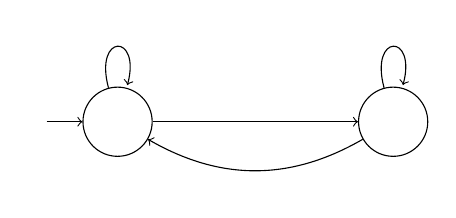
\begin{tikzpicture}[->, auto, node distance = 3.5cm]
			\node [state, initial left, initial text = ] (A) {};
			\node [state , right of = A] (B) {};
\path 	(A) edge [loop above] node {} (A)
				(B) edge [loop above] node {} (B)
				(A) edge node [above] {} (B)
				(B) edge [bend left] node [below] {} (A);
		\end{tikzpicture}
	\end{center}
\textbf{Automaton 2:} wsMNWA  with 
	\begin{center}
		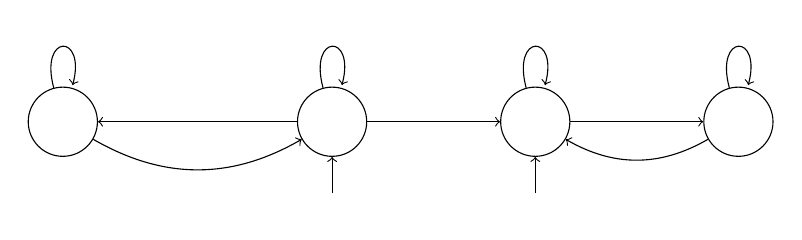
\begin{tikzpicture}[->, auto, node distance = 2.58cm]
			\node [state, initial below, initial text = ] (P) {};
			\node [state, initial below, initial text =, right of = P ] (A) {};
			\node [state, left of = P, xshift=-0.84cm] (Q) {};
			\node [state , right of = A] (B) {};
\path 	(A) edge [loop above] node {} (A)
				(B) edge [loop above] node {} (B)
				(P) edge [loop above] node {} (P)
				(P) edge node [above] {} (A)
				(A) edge node [above] {} (B)
				(B) edge [bend left] node [below] {} (A)
				(Q) edge [loop above] node {} (Q)
				(P) edge node [above] {} (Q)
				(Q) edge [bend right] node [below] {} (P);
		\end{tikzpicture}
	\end{center}
\end{example}
As usual, we extend the operation  and  to series  by means of pointwise definitions as follows:

We let  also denote the constant series with value , i.e.  for each .
For , we define the \emph{characteristic series}  by letting  if , and  otherwise.
We call a series  a \emph{regular step function} if

where  are regular languages of nested--words
	forming a partition of  and  for each ; so
	 iff 
	for each .
\par
An -pv-monoid  is \emph{regular} if for any alphabet  we have: For each  there exists a wsMNWA  with . Analogously to Droste and Meinecke \cite{DM} we can show that every left-distributive -pv-monoid is regular. \begin{Satz}
\label{rsfreg}
	Let  be a regular -pv-monoid. Then each regular step function  is regular. Furthermore, the set of all regular step functions is closed under  and .
\end{Satz}
Next we show that regular series are closed under projections. Consider a mapping  between two alphabets. Then  extends uniquely to an homomorphism between  and , also denoted by . Hence  is length-preserving and we can extend  to a function  by defining  for each .
Let  be a series. Then we define  for each  by

\begin{Satz}
	\label{hom}
	Let  be an -valuation monoid,  regular and . Then  is regular.
\end{Satz}
\section{Weighted MSO-Logic for Nested -Words} \label{kapMSOD}
In this section, we will present different fragments of our weighted MSO logic, and we give our first main result on the equivalence of these fragments. 
In the following  is always an -pv-monoid. We combine ideas of Alur and Madhusudan \cite{AM}, Droste and Gastin \cite{DG}, and Bollig and Gastin \cite{BG}, 
and divide the syntax of the weighted logic into a boolean part and a weighted part.
\begin{Def}[Syntax]
	The weighted monadic second order logic for nested words  is given by the following syntax
	
where ,~ and , ,  are first resp. second order variables. We call all formulas  \emph{boolean formulas}.
\end{Def}
The set of all positions of  is . Let . We denote the set of free variables of  by . Let  be a finite set of variables containing . As usual, we define a \emph{-assignment}  as function assigning to every first order variable of  a position of  and to every second order variable a subset of positions of .
We let
 (resp. ) be the -assignment (resp. )-assignment) mapping  to  (resp.  to ) and equaling  anywhere else. \par
We encode a pair  as nested -word as usual over the extended alphabet  with the same matching relation  (cf. \cite{DG}, \cite{DP}). We call  \emph{valid} if  emerges from a -assignment. Clearly the language  of all valid words is regular. \begin{Def}[Semantics]
\label{tab}
The semantics of  is a series . If  is not valid, we set . Otherwise we define \\  for  inductively as follows:
\begin{small}
	
	\vspace{-16pt}				
	\end{small}	\end{Def}
We write  for , so
	.
If  contains no free variables,  is a \emph{sentence} and
	.
\begin{example}
Continuing Example \ref{example:series} with  we define 
where . Then .
\end{example}
\par Analogously to \cite{DG} and \cite{DP} we can show:
\begin{Satz}
\label{prop:consistency}
	Let  and let  be a finite set of variables with . Then  for each valid . Furthermore,  is regular iff  is regular. 
\end{Satz}
\par
Clearly, every boolean formula  can be interpreted as an unweighted MSO-formula  with , since  only yields the values  and .
Conversely, for every formula  there exists a boolean MSO-formula  with , since we can replace disjunctions by conjunctions and negations and we can replace existential quantifiers by universal quantifiers and negations.
\par
In order to obtain a B\"uchi-like theorem (as Theorem \ref{main} below) for weighted automata on finite words, it is necessary to restrict the weighted MSO logic (cf. \cite{DG}). Therefore we introduce and study suitable fragments of  as in the following.
\begin{Def}
	The \emph{set of almost boolean formulas} is the smallest set of all formulas of  containing all constants  and all boolean formulas, which is closed under disjunction and conjunction.
\end{Def}
\begin{Satz}
	\label{almboolrsf}\begin{enumerate}[\quad (a)]
	\item If  is an almost boolean formula, then  is a regular step function.
	\item For every regular step function , there exists an almost boolean sentence  with .
	\end{enumerate}
\end{Satz}

\begin{Def}Let . We denote by  the set of all elements of  occurring in . We call 
	\begin{enumerate}
		\item \emph{strongly--restricted} if for all subformulas  of : \\
		Either  and  are almost boolean or  is boolean or  is boolean.
		\item \emph{-restricted} if for all subformulas  of : \\
 		Either  is almost boolean or  is boolean.
		\item \emph{commutatively--restricted} if for all subformulas  of : \\
 		Either  and  commute or  is almost boolean. \item \emph{-restricted} if for all subformulas  of :  is almost boolean.
	\end{enumerate}
\end{Def}
We call a formula of  \emph{syntactically restricted} if it is both -restricted and strongly--restricted. Note that every subformula of a syntactically restricted formula is syntactically restricted itself.
~\par
Now we show that under suitable assumptions on the -pv-monoid , particular classes of -formulas have the same expressive power. In \cite{DM} these equivalences (for unnested words) followed from the main result and thus needed constructions of automata. Here we show the equivalence of the logic fragments directly.
\begin{Theorem}
	\label{thm:restrict}
	\begin{enumerate}[\quad(a)]
		\item Let  be left-distributive and  be -restricted. Then there exists a strongly--restricted formula \\  with . Moreover, if  is also -restricted, then  can also be chosen to be -restricted.
		\item Let  be a cc--valuation semiring and let  be commutatively--restricted. Then there exists a strongly--restricted formula
 with . Moreover, if  is also -restricted, then  can also be chosen to be -restricted.
	\end{enumerate}
\end{Theorem}
\begin{proof}[Proof (sketch)]
	We use an induction on the structure of . The interesting case is  and  is almost boolean.
By induction we can assume that  and  are strongly--restricted (and resp. -restricted).
As an example,
we consider the case of the universal quantification in  as follows.
Assume  and  does not contain .
By the induction hypothesis, we obtain a strongly--restricted formula  such that .
\par 
First let  be left--distributive. Using this assumption at equation *, we get for  and each :

So  is strongly--restricted and .
If  is -restricted,  is almost boolean. In this case we can put directly . Then  is strongly--restricted and -restricted because  and  are almost boolean formulas.
\par
Now let  be left-multiplicative.
Using the formulas  and  it can be shown that

Then  is strongly--restricted since  is boolean. Furthermore,
.
If  is -restricted, we can put directly . Then  is strongly--restricted and -restricted because  and  are almost boolean formulas.
\end{proof}
If  is a cc--valuation semiring, clearly
 almost boolean formulas can be written as disjunctions
 of conjunctions of boolean formulas or constants from .
 Our proof of Theorem \ref{thm:restrict}  shows the following corollary.
\begin{Folgerung}
 Let  be a commutative cc--valuation semiring.
 Then for any formula  there exists a formula  in which conjunctions occur
 only between boolean formulas and constants such that .
\end{Folgerung}
 This follows also from a slightly modified proof of Theorem \ref{main},
 but the present proof gives direct and efficient
 conversions of the formulas.
\section{Characterization of Regular Series} \label{chapchar}
In this section, we give our second main result on the expressive equivalence of weighted stair Muller nested word automata and our different fragments of weighted MSO logic. 
\begin{Theorem}
\label{main}
	Let  be a regular -pv-monoid and  a series.
	\begin{enumerate}\item 	The following are equivalent:
		\begin{enumerate}\item .
			\item .
		\end{enumerate}
	\item 	Let  be left-distributive. Then the following are equivalent:
		\begin{enumerate}\item .
			\item \forall\wedge.
		\end{enumerate}
	\item 	Let  be cc--valuation semiring. Then the following are equivalent:
		\begin{enumerate}\item .
			\item \forall\wedge.
		\end{enumerate}
	\end{enumerate}
\end{Theorem}
\begin{proof}
\par 
\textbf{'':} We construct a syntactically restricted MSO-sentence simulating the given wsMNWA, thus showing all three statements. 
\par
\textbf{'':} By Theorem \ref{thm:restrict} we may assume  to be syntactically restricted. We prove the regularity of  by induction on the structure of  as follows.
If  is almost boolean, by Propositions \ref{almboolrsf}(a) and \ref{rsfreg},  is regular. Next we have to prove that the regularity is preserved under the non-boolean operations.
We only sketch the ideas. Closure under disjunction follows from Proposition \ref{hom} and a union construction of automata. If  is a conjunction, the regularity of  
follows from a product construction of automata. The regularity of  and  follows from Proposition \ref{hom}. For ,  is almost boolean. Then  can also be shown to be regular. \end{proof} 

	\section{Conclusion} 
We have introduced a weighted automaton model for infinite nested
words and weighted MSO logics. We could show that under suitable
assumptions on the valuation monoids, two resp. three fragments of the weighted logics have the same
expressive power with efficient conversions into the smallest
fragment. Moreover, the weighted automata and our logic fragments
have the same expressive power. The valuation monoids
form very general weight structures; they model
long-time average and discounted computations of weights as well
as the classical complete semirings \cite{DG}. As in \cite{AM}, we considered
nested words possibly containing pending edges. We remark that
our results also hold similarly for finite nested words, and our conversions of the weighted logic formulas also work, similarly, for other discrete structures like trees, cf. \cite{DGMM}. 

It would be interesting to investigate decision problems for
weighted nested word automata, e.g., like done in \cite{CDH}, \cite{CDH2} 
for automata on words and with average or discounted computations
of weights.\bibliography{sdbib}{}
\bibliographystyle{splncs03}
\end{document}
